\documentclass[12pt]{article}
\usepackage[utf8]{inputenc}
\usepackage{ulem}
\usepackage[english,russian]{babel}
\usepackage{amssymb}
\usepackage{graphicx}
\usepackage{setspace}
\usepackage{geometry}
\usepackage[english]{blindtext}
\usepackage[matrix,arrow,curve,frame,poly,arc]{xy}
\usepackage{fancyhdr}
\usepackage{subcaption}
\usepackage[export]{adjustbox}
\usepackage{wrapfig}
\usepackage{amsmath}
\usepackage{subfig}
\usepackage{hyperref}
\graphicspath{ {image} }
\hypersetup{pdfstartview=FitH,  linkcolor=linkcolor,urlcolor=urlcolor, colorlinks=true}

\begin{document}

    \begin{titlepage}
        \thispagestyle{empty}
        \begin{center}
            \noindent\begin{minipage}{0.14\textwidth}
                         
\includegraphics[width=\linewidth]{image/madi_logo}
            \end{minipage}%
            \begin{minipage}{0.86\textwidth}
                \center{\small{\vspace{\baselineskip}}}
                \center{{МИНИСТЕРСТВО НАУКИ И ВЫСШЕГО ОБРАЗОВАНИЯ РОССИЙСКОЙ ФЕДЕРАЦИИ \\ федеральное бюджетное образовательное государственное учреждение высшего образования}
                    \center{{\hspace{1 cm}}}}
            \end{minipage}
            \small{\textbf{<<МОСКОВСКИЙ АВТОМОБИЛЬНО-ДОРОЖНЫЙ ГОСУДАРСТВЕННЫЙ ТЕХНИЧЕСКИЙ УНИВЕРСИТЕТ (МАДИ)>>}}\\
            \vspace{0.2 cm}
            \scriptsize{{\textbf{КАФЕДРА <<ВЫСШАЯ МАТЕМАТИКА>> }}}
            \vspace{\baselineskip}

            \small{\textbf{КУРСОВАЯ РАБОТА}}\\
            \vspace{0.2 cm}

            по дисциплине <<Численные методы>>
            на тему\\
            <<Решение уравнений, систем линейных уравнений, интегралов, задачи Коши с помощью численных методов. >>
        \end{center}

        \hfill \begin{minipage}{0.5\linewidth}
                   \textbf{Выполнил:}\\
                   Учебная группа 2бПМ\\
                   Акилин.Я.А\\
                   \textbf{Руководитель курсового проекта:
                   }\\
                   Старший преподаватель\\
                   Шильников Евгений Владимирович\\
                   Подпись \underline{\hspace{1cm}}\\
        \end{minipage}
        \vspace{1 cm}
        \begin{minipage}{0.45\linewidth}
            Курсовой проект защищен\\ с оценкой <<\underline{\hspace{1cm}}>>\\
            <<\underline{\hspace{0.7cm}}>> \underline{\hspace{2cm}} 2023 г.
        \end{minipage}
        \begin{minipage}{0.55\linewidth}
        \end{minipage}
        \vspace{5 cm}
        \center{Москва 2023}
    \end{titlepage}

    \tableofcontents
    \newpage


    \section{Введение}
    В современном мире численные методы играют важную роль в решении различных математических задач. Они позволяют нам приближенно находить решения, которые не всегда возможно получить аналитически. В данной курсовой работе мы рассмотрим применение численных методов для решения нескольких классических задач.

    Одной из таких задач является решение нелинейных уравнений. Нелинейные уравнения широко применяются в различных областях науки и техники, и их точное решение может быть сложной задачей. Мы рассмотрим графический метод определения корней уравнения, а также итерационные методы, такие как метод деления отрезка пополам, метод простой итерации и метод Ньютона, которые позволят нам найти численные решения с заданной точностью.

    Другой важной задачей, которую мы рассмотрим, является решение систем линейных уравнений (СЛАУ). СЛАУ возникают во многих областях науки и инженерии, и их решение является ключевым этапом в анализе и моделировании различных процессов. Мы изучим различные методы решения СЛАУ, которые позволят нам найти численные решения и рассмотреть их свойства.

    Для вычисления интегралов мы рассмотрим численные методы, такие как метод трапеций и метод Симпсона. Эти методы позволяют приближенно вычислить значения интегралов путем разбиения области интегрирования на под отрезки и аппроксимации значения функции на этих подотрезках. Кроме того, мы также оценим погрешности этих вычислений, что позволит нам оценить точность полученных результатов.

    Другим важным аспектом, который мы рассмотрим, является использование интерполяционных многочленов. Интерполяция позволяет нам приближенно находить значения функции на основе ее известных значений в некоторых точках. Мы будем использовать многочлены различных степеней для нахождения значений функции, заданной таблично. Это позволит нам провести анализ и сравнение различных интерполяционных подходов.

    Наконец, мы обратимся к решению задач Коши, которые возникают в области дифференциальных уравнений. Задачи Коши описывают развитие системы дифференциальных уравнений с заданными начальными условиями. Мы рассмотрим методы Эйлера, модифицированный метод Эйлера и метод Рунге-Кутты 4-го порядка для численного решения задач Коши. Кроме того, мы оценим погрешность решений, что поможет нам сделать выводы о точности и стабильности этих методов.

    В данной работе мы реализуем описанные методы на языке программирования Java. Благодаря численным методам, которые мы изучим, мы сможем приближенно решать различные математические задачи и получать результаты с требуемой точностью.

    \newpage


    \section{Описание реализации проекта}
    В данной главе мы рассмотрим структуру проекта и описание реализации численных методов для решения различных задач.
    Проект разделен на несколько папок, каждая из которых содержит реализацию методов для решения определенных задач.

    \subsection{Уравнение}
    В папке "Уравнения" содержатся файлы и классы, связанные с численными методами для решения нелинейных уравнений.
    Рассмотрим каждый метод подробнее:

    \subsubsection{Метод деления отрезка пополам}
    Здесь представлен код реализации метода деления отрезка пополам для решения нелинейных уравнений.
    Ниже приведен фрагмент кода, в котором происходит вычисление корня уравнения с использованием данного метода:

    \begin{verbatim}
     public static double bisection(String functionString, double EPS, double[] limits) throws ScriptException {
        Scanner scanner = new Scanner(System.in);

        double leftBoundary = limits[0];
        double rightBoundary = limits[1];

        double valueLeftBoundFunction = evaluate(functionString, leftBoundary);
        double valueRightBoundFunction = evaluate(functionString, rightBoundary);

        if (valueLeftBoundFunction * valueRightBoundFunction > 0) {
            System.out.println("На заданном интервале нет корней!");
            return Double.NaN; // Возвращаем NaN, чтобы показать, что корень не найден.
        }

        double x0 = (leftBoundary + rightBoundary) / 2;

        while (Math.abs(rightBoundary - leftBoundary) >= EPS) {
            double valueX0Function = evaluate(functionString, x0);

            if (valueRightBoundFunction * valueX0Function >= 0) {
                rightBoundary = x0;
            } else {
                leftBoundary = x0;
            }

            x0 = (leftBoundary + rightBoundary) / 2;
        }

        return x0;
    }
    \end{verbatim}

    \subsubsection{Метод простой итерации}
    Здесь представлен представлен код реализации метода простой итерации для решения нелинейных уравнений. Ниже приведен фрагмент кода, демонстрирующий использование данного метода:

    \begin{verbatim}
          public static double iteration(String functionString, double EPS, double[] limits) throws ScriptException {
            int i = 1;
            double x = evaluate(functionString, limits[0]);
            double x0 = evaluate(functionString, x);
    
            while (true) {
                if (Math.abs(x - x0) < EPS) {
                    return x0;
                }
                x = evaluate(functionString,x0);
                x0 = evaluate(functionString,x0);
                i++;
    
                if (i == 10000) {
                    System.out.println("Выполнено 10000 итераций, решение не найдено!");
                    return Double.NaN;
                }
            }
        }
    \end{verbatim}

    \subsubsection{Метод Ньютона}
    Здесь представлен представлен код реализации метода Ньютона для решения нелинейных уравнений. Вот фрагмент кода, демонстрирующий использование данного метода:

    \begin{verbatim}
      public static double secant(String functionString,double EPS,double[] limits) throws ScriptException {
        String firstDerivative = Derivative.takeDerivative(functionString);
        String secondDerivative = Derivative.takeDerivative(firstDerivative);

        double leftBoundary = limits[0];
        double rightBoundary = limits[1];

        double valueLeftBoundFunction = evaluate(functionString, leftBoundary);
        double valueRightBoundFunction = evaluate(functionString, rightBoundary);

        double valueLeftBoundFirstDerivative = evaluate(firstDerivative, leftBoundary);
        double valueRightBoundFirstDerivative = evaluate(firstDerivative, rightBoundary);

        double valueLeftBoundSecondDerivative = evaluate(secondDerivative, leftBoundary);
        double valueRightBoundSecondDerivative = evaluate(secondDerivative, rightBoundary);

        double x0;

        if (valueLeftBoundFunction * valueLeftBoundSecondDerivative > 0){
            x0 = leftBoundary;
        }else if (valueRightBoundFunction * valueRightBoundSecondDerivative > 0){
            x0 = rightBoundary;
        }else {
            System.out.println("Неверно выбран начальный интревал!");
            return Double.NaN;
        }

        double x = x0 - (evaluate(functionString,x0) / evaluate(firstDerivative,x0));
        while(Math.abs(x - x0) >= EPS){
            x0 = x - (evaluate(functionString,x)/evaluate(firstDerivative,x));
            x = x0 - (evaluate(functionString,x0)/evaluate(firstDerivative,x0));
        }
        return x;
    }
    \end{verbatim}

    \subsubsection{Меню и ввод результатов}
    Для удобства использования и демонстрации работы численных методов, в проекте реализовано меню, которое позволяет выбирать нужный метод и вводить необходимые значения.


    Чтобы применить один из численных методов для решения уравнения $f(x) = x^3 - 2x + 2=0$, пользователь выбирает соответствующий метод из меню и вводит значения параметров, таких как точность ($\varepsilon$) и область поиска решения ($limits$).

    После ввода значений метод запускается и вычисляет решение уравнения с заданной точностью и областью поиска. Результат работы метода отображается на экране, позволяя оценить полученное решение.

    Таким образом, меню и ввод результатов предоставляют удобный интерфейс для работы с численными методами и исследования уравнения $f(x) = x^3 - 2x + 2=0$.

    \subsubsection{Прочие детали реализации}
    В этой части мы рассмотрим некоторые дополнительные детали реализации численных методов для решения уравнений:

    \textbf{Аргументы методов:}
    \begin{itemize}
        \item \texttt{functionString} -- строка, представляющая математическую функцию, передаваемую в метод. Она может содержать различные математические операции, переменные и константы.
        \item \texttt{EPS} -- точность, с которой методы должны найти решение уравнения. Значение \texttt{EPS} определяет требуемую близость результата к истинному значению решения.
        \item \texttt{limits} -- массив, указывающий границы области, в которой ищется решение уравнения. Обычно это два значения, представляющие левую и правую границы интервала.
    \end{itemize}

    \textbf{Методы \texttt{createFunction} и \texttt{evaluate}:}
    \begin{itemize}
        \item \texttt{createFunction} -- этот метод преобразует переданную математическую функцию, заданную в виде строки, во внутренний формат, понятный для программы. Он обеспечивает корректное вычисление значения функции.
        \item \texttt{evaluate} -- данный метод принимает функцию и значение аргумента и вычисляет значение функции в заданной точке. Он используется для получения значений функции при решении уравнений.
    \end{itemize}

    \textbf{Метод \texttt{takeDerivative}:}
    Для некоторых методов необходимо вычислять производную функции. В проекте реализован метод \texttt{takeDerivative}, который вычисляет значение производной переданной функции в заданной точке. Это позволяет использовать численные методы, требующие вычисления производной.

    Учет этих деталей реализации помогает эффективно применять численные методы для решения уравнений и получать точные результаты.

    \subsubsection{Результаты методов для решения уравнений}
    В данной части представлены результаты численных методов для решения уравнения, а также графическое решение уравнения.

    \paragraph{Описание функции:}
    Для иллюстрации работы численных методов мы рассмотрим уравнение $f(x) = x^3 - 2x + 2=0$. Именно это уравнение будет использоваться в дальнейшем для применения различных численных методов.

    Функция $f(x) = x^3 - 2x + 2=0$ представляет собой кубическую функцию с коэффициентами $a = 1$, $b = -2$ и $c = 2$. Наша задача состоит в нахождении корней этого уравнения с помощью численных методов, чтобы найти точные значения $x$, при которых $f(x) = 0$.

    Далее мы будем применять методы для нахождения корней данной функции и сравнивать результаты каждого метода.

    \paragraph{Графическое решение уравнения:}
    Прежде чем рассмотреть показания численных методов, давайте визуализируем уравнение графически. Ниже представлен график функции, где мы ищем решение уравнения:

    \clearpage

    \begin{figure}[h]
        \centering
        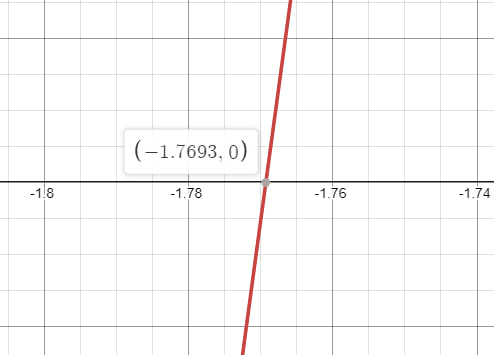
\includegraphics[width=0.6\textwidth]{image/graph_equation}
        \caption{Графическое решение уравнения}
    \end{figure}

    \paragraph{Результаты методов:}

    Теперь рассмотрим результаты работы каждого из трех численных методов: метода деления отрезка пополам, метода простой итерации и метода Ньютона. Ниже представлены фотографии с результатами работы каждого метода:

    \begin{figure}
        \centering
        \begin{subfigure}{0.4\textwidth}
            \centering
            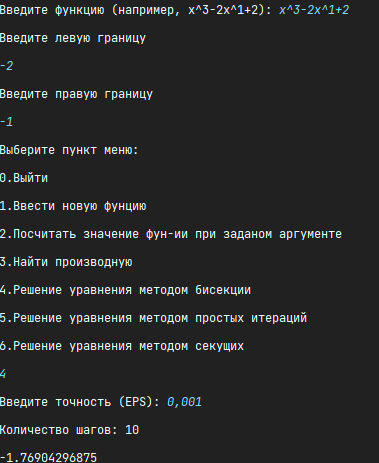
\includegraphics[width=\textwidth]{image/bisection_method}
            \caption{Метод деления отрезка пополам}
        \end{subfigure}
        \hfill
        \begin{subfigure}{0.4\textwidth}
            \centering
            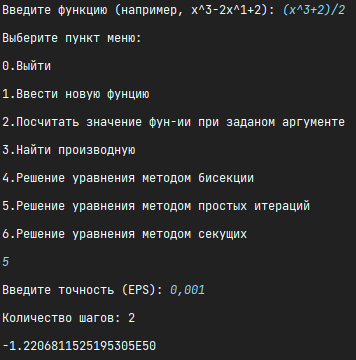
\includegraphics[width=\textwidth]{image/simple_iteration_method}
            \caption{Метод простой итерации}
        \end{subfigure}
        \hfill
        \begin{subfigure}{0.4\textwidth}
            \centering
            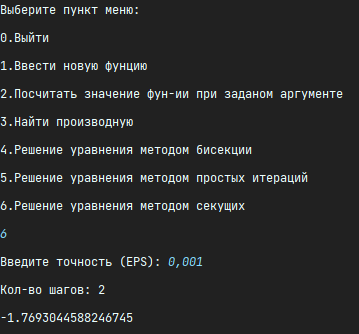
\includegraphics[width=\textwidth]{image/newton_method}
            \caption{Метод Ньютона}
        \end{subfigure}
        \caption{Результаты работы численных методов}
    \end{figure}

    Эти результаты наглядно демонстрируют эффективность и точность каждого из трех методов при решении данного уравнения.

    \clearpage

    \paragraph{Таблица с результатами:}
    Теперь занесем полученные данные в таблицу, что увидеть какой метод работает эффективнее.

    \begin{table}[h]
        \centering
        \begin{tabular}{|c|c|c|c|}
            \hline
            \textbf{Методы}               & \textbf{Результат} & \textbf{Погрешность}  & \textbf{Шагов} \\
            \hline
            Метод деления отрезка пополам & -1.769042968751     & 2.5703124900000596E-4 & 10             \\
            \hline
            Метод простой итерации        &-1.2206811525195305E50 &  1.2206811525195305E50  & 2              \\
            \hline
            Метод Ньютона                 & -1.7693044588246745 & 4.4588246743693105E-6 & 2              \\
            \hline
        \end{tabular}
        \caption{Итоги показаний методов}
    \end{table}

    \newpage

    \subsection{Система линейных уравнений}

    В данном разделе представлена система линейных уравнений, а также численные методы для ее решения. В проекте используются метод Гаусса и метод Зейделя.

    \subsubsection{Методы решения системы линейных уравнений}

    В проекте реализованы два численных метода для решения системы линейных уравнений: метод Гаусса и метод Зейделя.

    \paragraph{Метод Гаусса:}

    Метод Гаусса используется для решения систем линейных уравнений путем приведения их к упрощенной ступенчатой форме. Результатом метода Гаусса является точное решение системы.

    Ниже представлен фрагмент кода, в котором происходит вычисление решения системы с использованием данного метода:

    \begin{verbatim}
 public static double[] gauss(LinearSystem system) {
        int size = system.getSize();
        double[][] coefficients = system.getCoefficients();
        double[] rightHandSide = system.getRightHandSide();

        // Прямой ход
        for (int i = 0; i < size - 1; i++) {
            for (int j = i + 1; j < size; j++) {
                double ratio = coefficients[j][i] / coefficients[i][i];
                for (int k = i; k < size; k++) {
                    coefficients[j][k] -= ratio * coefficients[i][k];
                }
                rightHandSide[j] -= ratio * rightHandSide[i];
            }
        }

        // Обратный ход
        double[] solution = new double[size];
        for (int i = size - 1; i >= 0; i--) {
            double sum = 0.0;
            for (int j = i + 1; j < size; j++) {
                sum += coefficients[i][j] * solution[j];
            }
            solution[i] = (rightHandSide[i] - sum) / coefficients[i][i];
        }

        return solution;
    }
    \end{verbatim}

    \paragraph{Метод Зейделя:}
    Другим методом, который мы применим для решения системы линейных уравнений, является метод Зейделя. Вот фрагмент кода, в котором реализовано вычисление решения системы с использованием данного метода:

    \begin{verbatim}
 public static double[] seidel(LinearSystem system, double epsilon) {
        int maxIterations = 100000;
        int size = system.getSize();
        double[][] coefficients = system.getCoefficients();
        double[] rightHandSide = system.getRightHandSide();

        double[] solution = new double[size];
        double[] prevSolution = new double[size];
        int iteration = 0;

        while (iteration < maxIterations) {
            for (int i = 0; i < size; i++) {
                prevSolution[i] = solution[i];
            }

            for (int i = 0; i < size; i++) {
                double sum = 0.0;
                for (int j = 0; j < size; j++) {
                    if (j != i) {
                        sum += coefficients[i][j] * solution[j];
                    }
                }
                solution[i] = (rightHandSide[i] - sum) / coefficients[i][i];
            }

            double maxDiff = calculateNormDifference(solution, prevSolution); // Используем метод calculateNormDifference для расчета разности

            if (maxDiff < epsilon) {
                break;
            }

            iteration++;
        }

        return solution;
    }
    \end{verbatim}

    \subsubsection{Прочие детали реализации}

    При использовании метода Гаусса и метода Зейдаля для решения системы линейных уравнений пользователь будет вводить коэффициенты каждого уравнения для левой и правой частей. Для начала, пользователь должен указать размер системы, то есть количество уравнений.

    Из полученных данных будет создан объект системы, используя реализацию класса \texttt{LinearSystem}. Класс \texttt{LinearSystem} включает в себя:

    \begin{itemize}
        \item \texttt{coefficients}: двумерный массив, содержащий коэффициенты системы линейных уравнений.
        \item \texttt{rightHandSide}: одномерный массив, содержащий значения правой части уравнений.
    \end{itemize}

    Для создания объекта системы из введенных пользователем данных необходимо использовать методы класса \texttt{LinearSystem}. Одним из таких методов является \texttt{readSystemFromManualInput()}, который позволяет пользователю вводить коэффициенты и значения правой части системы вручную.

    Таким образом, после ввода данных и создания объекта системы, вы можете передать этот объект в ваши методы решения системы линейных уравнений, такие как метод Гаусса или метод Зейдаля.

    \clearpage

    \begin{figure}[ht]
        \centering
        {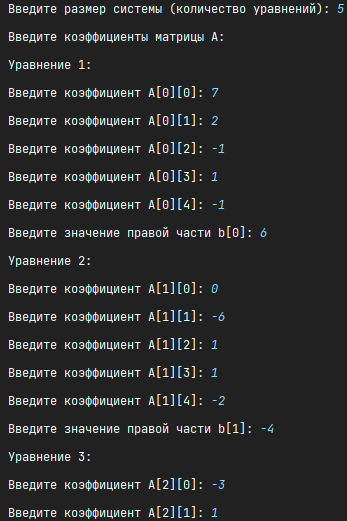
\includegraphics[width=0.4\textwidth]{image/system_input1}}
        \hfill
        {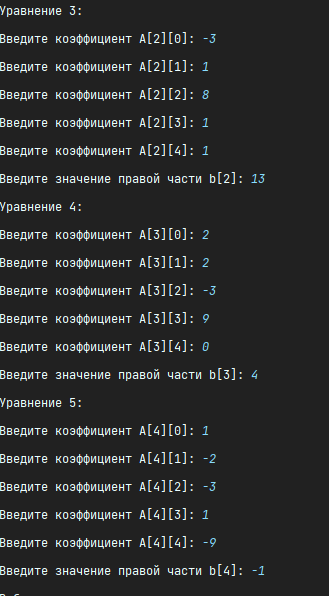
\includegraphics[width=0.4\textwidth]{image/system_input2}}
        \hfill
        {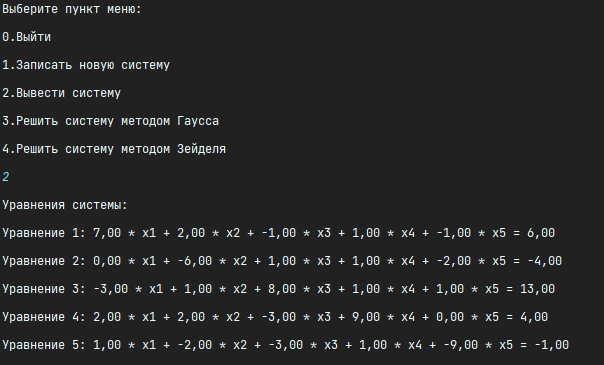
\includegraphics[width=0.4\textwidth]{image/system_input3}}
        \caption{Ввод данных для системы линейных уравнений}
    \end{figure}

    \subsubsection{Результаты методов для систем линейных уравнений}

    \paragraph{Описание системы линейных уравнений:}

    Рассмотрим систему линейных уравнений, состоящую из пяти уравнений:

    \begin{center}
        \[
            \begin{cases}
                7x_1 + 2x_2 - x_3 + x_4 - x_5 = 6 \\
                0x_1 - 6x_2 + x_3 + x_4 - 2x_5 = -4 \\
                -3x_1 + x_2 + 8x_3 + x_4 + x_5 = 13 \\
                2x_1 + 2x_2 - 3x_3 + 9x_4 = 4 \\
                x_1 - 2x_2 - 3x_3 + x_4 - 9x_5 = -1 \\
            \end{cases}
        \]
    \end{center}

    Эта система состоит из пяти уравнений с пятью неизвестными: $x_1, x_2, x_3, x_4, x_5$. Коэффициенты перед неизвестными и правые части уравнений указаны выше.

    \paragraph{Результаты методов:}

    Теперь рассмотрим результаты работы двух численных методов: метода Гаусса и метода Зейдаля. Ниже представлены скриншоты с показаниями и работой каждого метода.

    \begin{figure}[ht]
        \centering
        \begin{subfigure}{0.4\textwidth}
            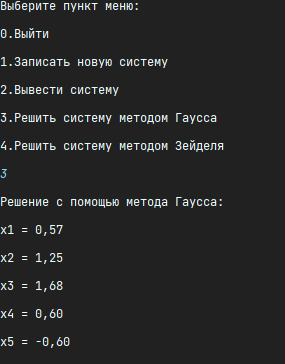
\includegraphics[width=\linewidth]{image/gauss_equation}
            \caption{Результат работы метода Гаусса}
        \end{subfigure}
        \hfill
        \begin{subfigure}{0.4\textwidth}
            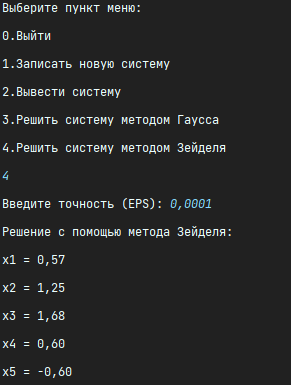
\includegraphics[width=\linewidth]{image/zeidel_equation}
            \caption{Результат работы метода Зейдаля}
        \end{subfigure}
        \caption{Результаты работы методов для уравнений}
    \end{figure}

    \paragraph{Таблица с результатами:}

    Затем можно создать таблицу, в которую вы сможете вносить полученные данные для уравнений:

    \begin{table}[ht]
        \centering
        \begin{tabular}{|c|c|c|c|c|c|}
            \hline
            \textbf{Метод} & \multicolumn{5}{c|}{\textbf{Результаты}} \\
            \hline
            & $x_1$ & $x_2$ & $x_3$ & $x_4$ & $x_5$ \\
            \hline
            Метод Гаусса  & 0,57  & 1,25  & 1,68  & 0,60  & -0,60 \\
            \hline
            Метод Зейделя & 0,57  & 1,25  & 1,68  & 0,60  & -0,60 \\
            \hline
        \end{tabular}
        \caption{Результаты работы методов для уравнений}
    \end{table}

    \subsection{Вычисление интеграла}

    В данной подсекции мы рассмотрим численные методы для вычисления определенного интеграла. Для иллюстрации применимости данных методов, рассмотрим конкретный пример с подынтегральной функцией $f(x) = x^3 - 2x +2$ и пределами интегрирования от 1 до 2.2.

    \subsubsection{Метод трапеций}

    Метод трапеций является одним из простейших численных методов для вычисления интегралов. Он основан на аппроксимации подынтегральной функции с помощью линейных отрезков, образованных верхними и нижними трапециями.

    Ниже приведен пример кода, реализующего метод трапеций для вычисления интеграла:

    \begin{verbatim}
  public static double integrateByTrapezoidRule(String functionString, double[] limits, int n) throws ScriptException, ScriptException {
        double a = limits[0];
        double b = limits[1];

        DoubleUnaryOperator function = createFunction(functionString);
        double h = (b - a) / n;
        double sum = 0.5 * (function.applyAsDouble(a) + function.applyAsDouble(b));
        for (int i = 1; i < n; i++) {
            double x = a + i * h;
            sum += function.applyAsDouble(x);
        }
        return h * sum;
    }
    \end{verbatim}

    \subsubsection{Метод Симпсона}

    Метод Симпсона является более точным численным методом для вычисления интегралов. Он основан на аппроксимации подынтегральной функции с помощью парабол, проходящих через три точки.

    Ниже приведен пример кода, реализующего метод Симпсона для вычисления интеграла:

    \begin{verbatim}
 public static double integrateBySimpsonRule(String functionString, double[] limits, int n) throws ScriptException, ScriptException {
        double a = limits[0];
        double b = limits[1];

        if (n % 2 != 0) {
            throw new IllegalArgumentException("Number of intervals (n) must be even for Simpson's rule.");
        }
        DoubleUnaryOperator function = createFunction(functionString);
        double h = (b - a) / n;
        double sum = function.applyAsDouble(a) + function.applyAsDouble(b);
        for (int i = 1; i < n; i++) {
            double x = a + i * h;
            sum += (i % 2 == 0) ? 2 * function.applyAsDouble(x) : 4 * function.applyAsDouble(x);
        }
        return h / 3 * sum;
    }
    \end{verbatim}

    \subsubsection{Вычисление погрешности с использованием правила Рунге}

    Правило Рунге позволяет оценить погрешность численного метода, используя результаты вычислений с разными шагами. Ниже приведены примеры кода, демонстрирующие вычисление погрешности с использованием правила Рунге для метода трапеций и его усовершенствованной версии для метода Симпсона.

    Для метода трапеций:
    \begin{verbatim}
public static double estimateErrorByRungeRuleTrapezoid(String functionString, double[] limits, int n) throws ScriptException {
        double a = limits[0];
        double b = limits[1];

        // Вычисляем интеграл с более грубым разбиением
        int nCoarse = n / 2;
        double integralCoarse = integrateByTrapezoidRule(functionString, limits, nCoarse);

        // Вычисляем интеграл с более точным разбиением
        double integralFine = integrateByTrapezoidRule(functionString, limits, n);

        // Оцениваем погрешность решения по правилу Рунге
        return Math.abs(integralFine - integralCoarse) / (Math.pow(2, 2) - 1);
    }
    \end{verbatim}

    Для метода Симпсона:
    \begin{verbatim}
  public static double estimateErrorByRichardsonSimpson(String functionString, double[] limits, int n) throws ScriptException {
        double integral = integrateBySimpsonRule(functionString, limits, n);
        double integral2 = integrateBySimpsonRule(functionString, limits, 2 * n);

        double error = Math.abs((1 / 15.0) * (integral - integral2));

        return error;
    }
    \end{verbatim}

    \subsubsection{Результаты методов для вычисления интегралов}

    \paragraph{Результаты методов:}
    Теперь рассмотрим результаты работы двух численных методов: метода трапеций с использованием метода Рунге и метода Симпсона с использованием его усовершенствованной версии. Ниже представлены скриншоты с результатами работы каждого метода.

    \begin{figure}[ht]
        \centering
        \begin{subfigure}{0.4\textwidth}
            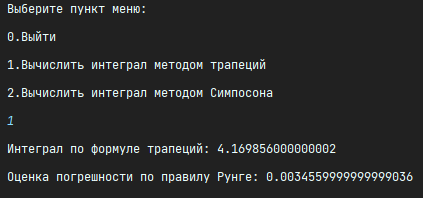
\includegraphics[width=\linewidth]{image/trapezoid_rule}
            \caption{Результат работы метода трапеций}
        \end{subfigure}
        \hfill
        \begin{subfigure}{0.4\textwidth}
            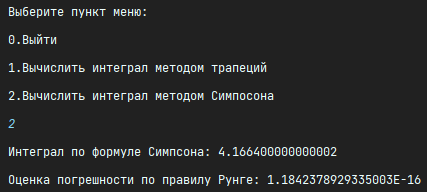
\includegraphics[width=\linewidth]{image/simpson_rule}
            \caption{Результат работы метода Симпсона}
        \end{subfigure}
        \caption{Результаты работы методов для интегралов}
    \end{figure}

    \paragraph{Таблица с результатами:}
    Затем можно создать таблицу, в которую вы сможете вносить полученные данные для каждого метода:

    \begin{table}[ht]
        \centering
        \begin{tabular}{|c|c|c|}
            \hline
            \textbf{Метод} & \textbf{Результат} & \textbf{Погрешность} \\
            \hline
            Метод трапеций & 4.169856000000002 & 0.0034559999999999036 \\
            \hline
            Метод Симпсона & 4.166400000000002 & 1.1842378929335003E-16 \\
            \hline
        \end{tabular}
        \caption{Результаты работы методов для интегралов}
    \end{table}

    \subsection{Вычисление значений функции с использованием интерполяционных многочленов}


    С помощью интерполяционных многочленов степени от 1 до 4, мы можем найти значения функции, заданной таблично, в точке $x_0 = 1.1$. Для этого мы будем использовать метод интерполяции, который позволяет аппроксимировать функцию на основе заданных точек.

    \subsubsection{Инициализация массивов данных}

    \begin{center}
        \begin{tabular}{|c|c|c|c|c|c|}
            \hline
            x & -1   & 0     & 1    & 2     & 3     \\
            \hline
            y & 20.8 & 15.9  & 14.8 & 17.96 & 15.06 \\
            \hline
        \end{tabular}
    \end{center}

    В моем проекте для инициализации этих значений, я использовал считывание данных из файлов. Для этого я создал два класса: InitArrayX и InitArrayY.

    В классе InitArrayX я реализовал методы fillArrayX и fillArrayXFromFile. Метод fillArrayX считывает значения для массива x с помощью класса Scanner из стандартного ввода. Метод fillArrayXFromFile считывает значения для массива x из файла, переданного в качестве аргумента. Он открывает файл, создает экземпляр Scanner для чтения данных из файла и построчно считывает значения в массив x.

    Аналогично, в классе InitArrayY я реализовал методы fillArrayY и fillArrayYFromFile для инициализации массива y. Эти методы также считывают значения из стандартного ввода или из файла.

    \begin{figure}[h]

        \centering

        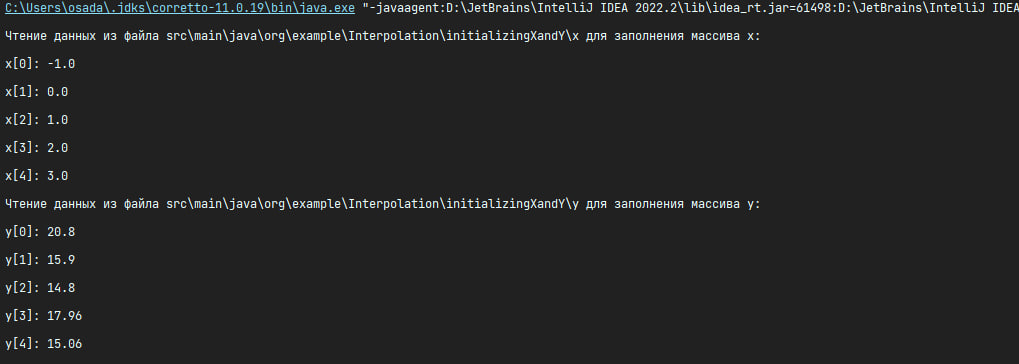
\includegraphics[width=0.8\linewidth]{image/initXandY}

        \caption{Заполнение массивовов x и y}

        \label{fig:mpr}

    \end{figure}

    \subsubsection{Интерполяционные многочлены}

    \paragraph{Метод \texttt{interpolateAndPrint}}
    Данный метод выполняет интерполяцию и выводит результаты для каждой степени от 1 до 4. Вот его код:

    \begin{verbatim}
public static void interpolateAndPrint(double x0, double[] x, double[] y) {
for (int degree = 1; degree <= 4; degree++) {
double result = interpolate(x0, x, y, degree);
System.out.println("Степень " + degree + ": " + result);
}
}
    \end{verbatim}

    \paragraph{Метод \texttt{interpolate}}
    Данный метод выполняет интерполяцию для заданной степени. Вот его код:

    \begin{verbatim}
public static double interpolate(double x0, double[] x, double[] y, int degree) {
int n = degree + 1;
int[] indices = getIndices(x, x0, n);
double[] xSubset = getSubset(x, indices);
double[] ySubset = getSubset(y, indices);
return computeInterpolation(x0, xSubset, ySubset, degree);
}
    \end{verbatim}

    \paragraph{Метод \texttt{getIndices}}
    Данный метод возвращает индексы элементов массива x, которые будут использоваться для интерполяции. Вот его код:

    \begin{verbatim}
private static int[] getIndices(double[] x, double x0, int n) {
int[] indices = new int[n];
int closestIndex = findClosestIndex(x, x0);
int startIndex = Math.max(0, closestIndex - n / 2);
for (int i = 0; i < n; i++) {
indices[i] = startIndex + i;
}
return indices;
}
    \end{verbatim}

    \paragraph{Метод \texttt{findClosestIndex}}
    Данный метод находит индекс элемента массива x, ближайшего к значению x0. Вот его код:

    \begin{verbatim}
private static int findClosestIndex(double[] x, double x0) {
int closestIndex = 0;
double closestDistance = Math.abs(x[0] - x0);
for (int i = 1; i < x.length; i++) {
double distance = Math.abs(x[i] - x0);
if (distance < closestDistance) {
closestIndex = i;
closestDistance = distance;
}
}
return closestIndex;
}
    \end{verbatim}

    \paragraph{Метод \texttt{getSubset}}
    Данный метод возвращает подмассив arr, состоящий из элементов с заданными индексами. Вот его код:

    \begin{verbatim}
private static double[] getSubset(double[] arr, int[] indices) {
double[] subset = new double[indices.length];
for (int i = 0; i < indices.length; i++) {
subset[i] = arr[indices[i]];
}
return subset;
}
    \end{verbatim}

    \paragraph{Метод \texttt{computeInterpolation}}
    Данный метод вычисляет интерполяцию для заданных значений x, y и степени. Вот его код:

    \begin{verbatim}
private static double computeInterpolation(double x0, double[] x, double[] y, int degree) {
double result = 0.0;
for (int i = 0; i <= degree; i++) {
double term = y[i];
for (int j = 0; j <= degree; j++) {
if (j != i) {
term *= (x0 - x[j]) / (x[i] - x[j]);
}
}
result += term;
}
return result;
}
    \end{verbatim}

    \subsubsection{Вычисление погрешности}

    \paragraph{Метод \texttt{computeErrors}}
    Данный метод вычисляет погрешность интерполяции для каждой степени от 1 до 4. Вот его код:

    \begin{verbatim}
public static void computeErrors(double x0, double[] x, double[] y) {
    for (int degree = 1; degree <= 4; degree++) {
        double interpolatedValue = interpolate(x0, x, y, degree);
        double trueValue = computeTrueValue(x0, x, y);

        double error = Math.abs(interpolatedValue - trueValue);
        System.out.println("Степень " + degree + ": Погрешность = " + error);
    }
}
    \end{verbatim}

    \paragraph{Метод \texttt{computeTrueValue}}
    Данный метод вычисляет истинное значение функции для заданного значения $x_0$. Вот его код:

    \begin{verbatim}
public static double computeTrueValue(double x0, double[] x, double[] y) {
    int index = findNearestIndex(x0, x);
    return y[index];
}
    \end{verbatim}

    \paragraph{Метод \texttt{findNearestIndex}}
    Данный метод находит индекс элемента массива $x$, ближайшего к значению $x_0$. Вот его код:

    \begin{verbatim}
public static int findNearestIndex(double x0, double[] x) {
    int index = 0;
    double minDiff = Math.abs(x0 - x[0]);

    for (int i = 1; i < x.length; i++) {
        double diff = Math.abs(x0 - x[i]);
        if (diff < minDiff) {
            minDiff = diff;
            index = i;
        }
    }

    return index;
}
    \end{verbatim}

    \subsubsection{Результаты работы методов с интерполяционными многочленами}

    \paragraph*{Результаты методов:}

    \clearpage

    \begin{figure}
        \centering
        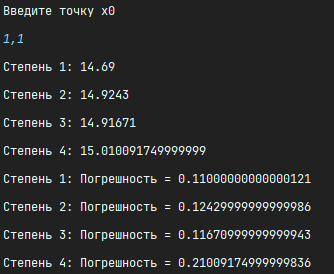
\includegraphics[width=\textwidth]{image/values_interpolate_plot}
        \caption{Значения функции при разных степенях интерполяционного многочлена}

    \end{figure}

    \clearpage
    \paragraph*{Таблица с результатами:}
    \begin{table}
        \centering
        \caption{Значения функции и погрешности при разных степенях многочлена}
        \begin{tabular}{|c|c|c|}
            \hline
            \textbf{Степень} & \textbf{Значение функции} & \textbf{Погрешность} \\
            \hline
            1                & 14.69                    & 0.11                 \\
            2                & 14.9243                  & 0.1243               \\
            3                & 14.91671                 & 0.11671              \\
            4                & 15.010091749999999       & 0.21009174999999836  \\
            \hline
        \end{tabular}
        \label{tab:results}
    \end{table}

    \subsection{Решение задачи Коши}

    Для решения задачи Коши с начальным условием $y(1)=0$ на отрезке $x=[1;2.2]$ с шагом $h=0.1$, мы использовали три численных метода: метод Эйлера, модифицированный метод Эйлера и метод Рунге-Кутты 4-го порядка.

    \subsubsection{Метод Эйлера}


    \begin{verbatim}
    public static Map<String, List<Double>> euler(String functionString, double[] limits, double h, double y0) throws ScriptException {
        List<Double> x1 = new ArrayList<>();
        List<Double> y1 = new ArrayList<>();

        double x0 = limits[0];
        double xLast = limits[1];

        x1.add(x0);
        y1.add(y0);

        DoubleBinaryOperator function = createFunction(functionString);

        int n = (int) Math.round((xLast - x0) / h);

        for (int i = 0; i < n; i++) {
            double f = evaluateFunctionTwoVariables(functionString, x0, y0);
            y0 = y0 + h * f;
            x0 = x0 + h;

            x1.add(x0);
            y1.add(y0);
        }

        Map<String, List<Double>> result = new HashMap<>();
        result.put("x1", x1);
        result.put("y1", y1);

        return result;
    }
    \end{verbatim}

    \subsubsection{Модифицированный метод Эйлера}

    \begin{verbatim}
    pu public static Map<String, List<Double>> modifiedEuler(String functionString, double[] limits, double h, double y0) throws ScriptException {
        List<Double> x1 = new ArrayList<>();
        List<Double> y1 = new ArrayList<>();

        double x0 = limits[0];
        double xLast = limits[1];

        x1.add(x0);
        y1.add(y0);

        int n = (int) Math.round((xLast - x0) / h);

        for (int i = 0; i < n; i++) {
            double f1 = evaluateFunctionTwoVariables(functionString, x0, y0);
            double xHalf = x0 + h / 2.0;
            double yHalf = y0 + h / 2.0 * f1;
            double f2 = evaluateFunctionTwoVariables(functionString, xHalf, yHalf);

            double yNext = y0 + h * f2;
            x0 = x0 + h;
            y0 = yNext;

            x1.add(x0);
            y1.add(y0);
        }

        Map<String, List<Double>> result = new HashMap<>();
        result.put("x1", x1);
        result.put("y1", y1);

        return result;
    }
    \end{verbatim}

    \subsubsection{Метод Рунге-Кутты 4-го порядка}

    \begin{verbatim}
    public static Map<String, List<Double>> rungeKutta4(String functionString, double[] limits, double h, double y0) throws ScriptException {
        List<Double> x1 = new ArrayList<>();
        List<Double> y1 = new ArrayList<>();

        double x0 = limits[0];
        double xLast = limits[1];

        x1.add(x0);
        y1.add(y0);

        int n = (int) Math.round((xLast - x0) / h);

        for (int i = 0; i < n; i++) {
            double k1 = evaluateFunctionTwoVariables(functionString, x0, y0);
            double k2 = evaluateFunctionTwoVariables(functionString, x0 + h / 2.0, y0 + h / 2.0 * k1);
            double k3 = evaluateFunctionTwoVariables(functionString, x0 + h / 2.0, y0 + h / 2.0 * k2);
            double k4 = evaluateFunctionTwoVariables(functionString, x0 + h, y0 + h * k3);

            double yNext = y0 + h / 6.0 * (k1 + 2 * k2 + 2 * k3 + k4);
            x0 = x0 + h;
            y0 = yNext;

            x1.add(x0);
            y1.add(y0);
        }

        Map<String, List<Double>> result = new HashMap<>();
        result.put("x1", x1);
        result.put("y1", y1);

        return result;
    }
    \end{verbatim}

    \subsubsection{Прочие детали реализации}

    Для использования методов Эйлера, модифицированного метода Эйлера и метода Рунге-Кутты 4-го порядка вам потребуется отдельный метод, который будет вычислять значение функции двух переменных:

    \begin{verbatim}
 // Вычисление значения функции при заданных аргументах x и y
    public static double evaluateFunctionTwoVariables(String functionString, double x, double y) throws ScriptException {
        DoubleBinaryOperator function = createFunction(functionString);
        try {
            return function.applyAsDouble(x, y);
        } catch (Exception ex) {
            ex.printStackTrace();
            throw ex;
        }
    }

    // Правильная обработка функции с двумя переменными x и y
    public static DoubleBinaryOperator createFunction(String function) throws ScriptException {
        function = function.replaceAll("(\\d+(,\\d+)?)\\^(\\d+)", "Math.pow($1, $3)");
        function = function.replaceAll("(\\d+(,\\d+)?)x", "$1*x");
        function = function.replaceAll("x\\^(\\d+)", "Math.pow(x, $1)");
        function = function.replaceAll("(\\d+(,\\d+)?)y", "$1*y");
        function = function.replaceAll("y\\^(\\d+)", "Math.pow(y, $1)");
        function = function.replaceAll("e", "2.7");
        ScriptEngineManager manager = new ScriptEngineManager();
        ScriptEngine engine = manager.getEngineByName("js");
        engine.eval("function f(x, y) { return " + function + "; }");
        Invocable invocable = (Invocable) engine;
        String finalFunction = function;
        return (x, y) -> {
            try {
                Object result = invocable.invokeFunction("f", x, y);
                if (result instanceof Number) {
                    return ((Number) result).doubleValue();
                } else {
                    throw new IllegalArgumentException("Function result is not a number");
                }
            } catch (ScriptException | NoSuchMethodException ex) {
                throw new IllegalArgumentException("Invalid function: " + finalFunction, ex);
            }
        };
    }
    \end{verbatim}

    Кроме того, для оценки погрешности этих методов вы используете правило Рунге-Ромберга. Ниже представлен код, который вы можете использовать для оценки погрешности:

    \begin{verbatim}
 public static double estimateErrorRungeRomberg(List<Double> solution, double h) {
        int n = solution.size();

        double error = 0.0;
        for (int i = 0; i < n - 1; i++) {
            double y1 = solution.get(i);
            double y2 = solution.get(i + 1);
            double exactValue = (y2 - y1) / (h);

            error += Math.pow(exactValue - y2, 2);
        }

        return Math.sqrt(error);
    }
    \end{verbatim}

    \subsubsection{Результаты методов для задачи Коши}

    \paragraph*{Результаты методов:}
    Теперь рассмотрим результаты работы трех численных методов: метода Эйлера, модифицированного метода Эйлера и метода Рунге-Кутты 4-го порядка для решения задачи Коши на заданном отрезке. Ниже приведены скриншоты с результатами работы каждого метода.

    \clearpage

    \begin{figure}[ht]
        \centering
        \begin{subfigure}{0.4\textwidth}
            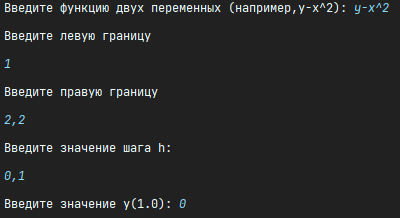
\includegraphics[width=\linewidth]{image/menu_Koshi}
            \caption{Меню}
        \end{subfigure}
        \begin{subfigure}{0.4\textwidth}
            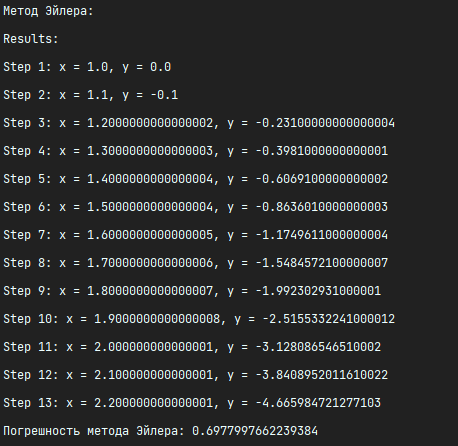
\includegraphics[width=\linewidth]{image/euler_method}
            \caption{Результат работы метода Эйлера}
        \end{subfigure}
        \hfill
        \begin{subfigure}{0.4\textwidth}
            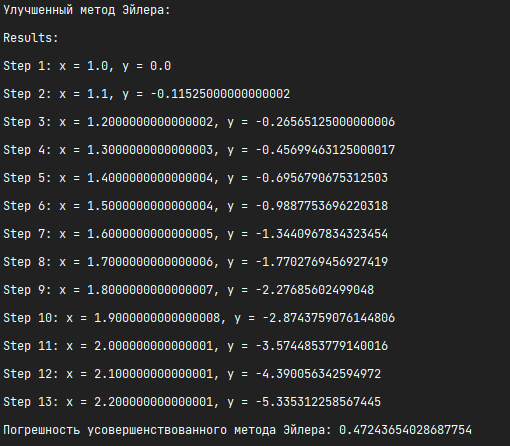
\includegraphics[width=\linewidth]{image/modified_euler_method}
            \caption{Результат работы модифицированного метода Эйлера}
        \end{subfigure}
        \hfill
        \begin{subfigure}{0.4\textwidth}
            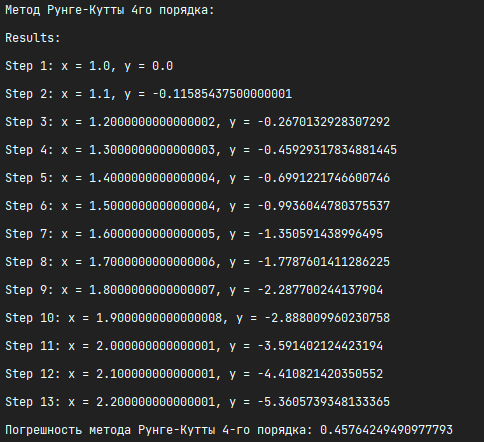
\includegraphics[width=\linewidth]{image/runge_kutta_method}
            \caption{Результат работы метода Рунге-Кутты 4-го порядка}
        \end{subfigure}
        \caption{Результаты работы методов для задачи Коши}
    \end{figure}

    \paragraph*{Графическое показание методов:}

    \begin{figure}[h]
        \centering
        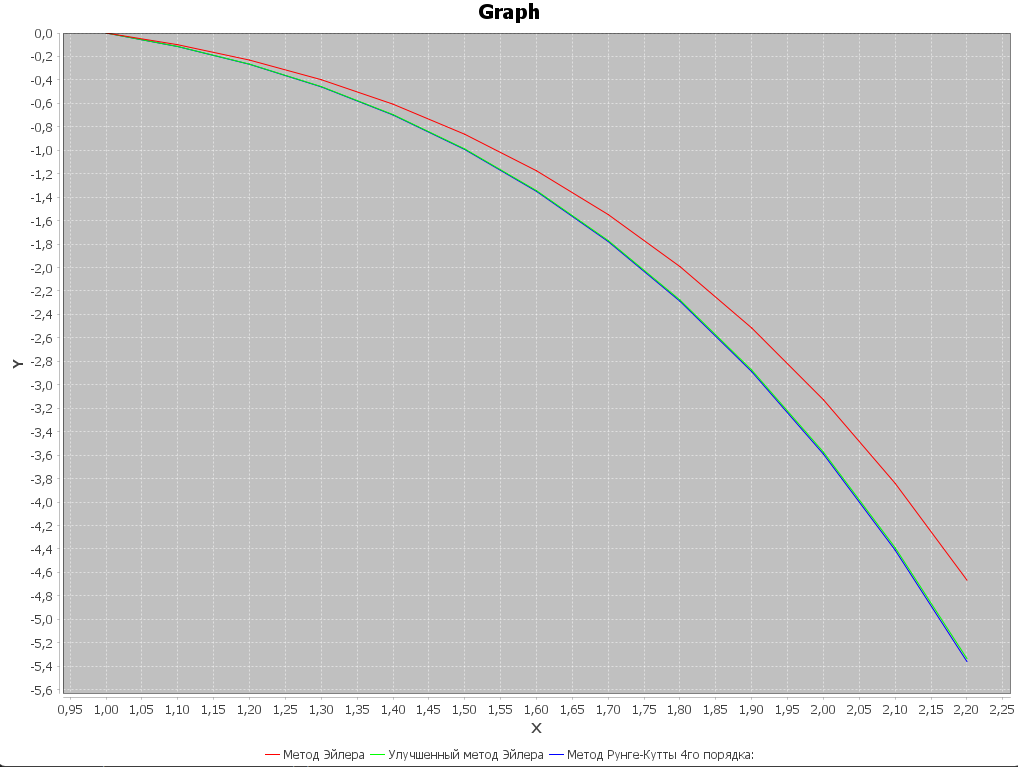
\includegraphics[width=0.8\textwidth]{image/graph_koshi}
        \caption{Графическое решение задачи Коши}
        \label{fig:graphical_solution}
    \end{figure}

    Затем можно создать таблицу, в которую вы сможете вносить полученные данные для каждого метода, включая значения и погрешности:

    \clearpage

    \begin{table}[h]
        \centering
        \caption{Результаты методов}
        \begin{tabular}{|c|c|c|c|}
            \hline
            \textbf{Шаг} & \textbf{Метод Рунге-Кутты 4} & \textbf{Метод Эйлера}  & \textbf{Улучшенный метод Эйлера} \\
            \hline
            1            & $x = 1.0, y = 0.0$           & $x = 1.0, y = 0.0$     & $x = 1.0, y = 0.0$               \\
            \hline
            2            & $x = 1.1, y = -0.116$         & $x = 1.1, y = -0.1$    & $x = 1.1, y = -0.115$            \\
            \hline
            3            & $x = 1.2, y = -0.267$         & $x = 1.2, y = -0.231$  & $x = 1.2, y = -0.266$            \\
            \hline
            4            & $x = 1.3, y = -0.459$         & $x = 1.3, y = -0.398$  & $x = 1.3, y = -0.457$            \\
            \hline
            5            & $x = 1.4, y = -0.699$         & $x = 1.4, y = -0.607$  & $x = 1.4, y = -0.696$            \\
            \hline
            6            & $x = 1.5, y = -0.994$         & $x = 1.5, y = -0.864$  & $x = 1.5, y = -0.989$            \\
            \hline
            7            & $x = 1.6, y = -1.351$         & $x = 1.6, y = -1.175$  & $x = 1.6, y = -1.344$            \\
            \hline
            8            & $x = 1.7, y = -1.779$         & $x = 1.7, y = -1.548$  & $x = 1.7, y = -1.770$            \\
            \hline
            9            & $x = 1.8, y = -2.288$         & $x = 1.8, y = -1.992$  & $x = 1.8, y = -2.277$            \\
            \hline
            10           & $x = 1.9, y = -2.888$         & $x = 1.9, y = -2.516$  & $x = 1.9, y = -2.874$            \\
            \hline
            11           & $x = 2.0, y = -3.591$         & $x = 2.0, y = -3.128$  & $x = 2.0, y = -3.574$            \\
            \hline
            12           & $x = 2.1, y = -4.411$         & $x = 2.1, y = -3.841$  & $x = 2.1, y = -4.390$            \\
            \hline
            13           & $x = 2.2, y = -5.361$         & $x = 2.2, y = -4.666$  & $x = 2.2, y = -5.335$            \\
            \hline
        \end{tabular}
    \end{table}


    \begin{table}[h]
        \centering
        \caption{Погрешности методов}
        \begin{tabular}{|c|c|}
            \hline
            \textbf{Метод}                 & \textbf{Погрешность} \\
            \hline
            Метод Эйлера                   & 0.025267741432554836              \\
            \hline
            Улучшенный метод Эйлера        & 0.6945952787228968          \\
            \hline
            Метод Рунге-Кутты 4-го порядка & 6.065186663128941E-6               \\
            \hline
        \end{tabular}
    \end{table}


    \section{Вывод}

    В ходе выполнения данной курсовой работы были рассмотрены и решены следующие задачи: определение корней уравнения, решение СЛАУ, вычисление интеграла и использование интерполяционных многочленов. Кроме того, была решена задача Коши с применением различных численных методов.

    Для определения корней уравнения графически была использована визуализация функции и выявление точек пересечения с осью абсцисс. Для уточнения одного из корней были применены итерационные методы: метод деления отрезка пополам, метод простой итерации и метод Ньютона. С помощью этих методов был достигнут заданный уровень точности в 0,001.

    Для решения СЛАУ были применены соответствующие алгоритмы, такие как метод Гаусса или метод прогонки, в зависимости от характеристик системы. Результаты решения системы линейных алгебраических уравнений позволили найти значения неизвестных переменных.

    Вычисление интеграла проводилось с использованием численных методов, таких как метод трапеций и метод Симпсона. Погрешности вычислений были оценены с помощью соответствующих методов, например, с использованием правила Рунге.

    Интерполяционные многочлены степени от 1 до 4 были использованы для нахождения значений функции в заданных точках. Погрешность была оценена с учетом выбранной степени многочлена и сравнения с исходными значениями функции.

    Наконец, задача Коши была решена с применением методов Эйлера, модифицированного метода Эйлера и метода Рунге-Кутты 4-го порядка. Результаты работы каждого метода были сопоставлены и погрешность была оценена с использованием правила Рунге Ромберга.

    В результате выполнения данной курсовой работы были получены численные значения корней уравнения, решения СЛАУ, интеграла, значений функции с использованием интерполяции, а также решение задачи Коши. Оценка погрешностей позволяет учесть точность и достоверность полученных результатов.

\end{document}